% File: solutions/ex24.tex
\begin{soluzione}{24}
    \begin{enumerate}
        \item \textbf{Trasformata di Fourier di $x(t)$}
        
        Il segnale è un prodotto: $x(t) = g(t) \cdot m(t)$, dove:
        \begin{itemize}
            \item $g(t) = \left( \frac{\sin(\pi t)}{\pi t} \right)^2 = \text{sinc}^2(t)$. La sua trasformata, come suggerito, è una funzione triangolare: $G(f) = \text{tri}(f)$, che è un triangolo di altezza 1 e base da -1 a 1 Hz.
            \item $m(t) = 1 - 2\cos(2\pi t)$. La sua trasformata $M(f)$ si calcola usando la linearità e la trasformata notevole del coseno:
            \[
                M(f) = \delta(f) - 2 \cdot \frac{1}{2}[\delta(f-1) + \delta(f+1)] = \delta(f) - \delta(f-1) - \delta(f+1)
            \]
        \end{itemize}
        La trasformata $X(f)$ è la convoluzione $G(f) * M(f)$:
 
        \begin{align*}
            X(f) &= \text{tri}(f) * [\delta(f) - \delta(f-1) - \delta(f+1)] \\
            &= (\text{tri}(f) * \delta(f)) - (\text{tri}(f) * \delta(f-1)) - (\text{tri}(f) * \delta(f+1)) \\
            &= \mathbf{\text{tri}(f) - \text{tri}(f-1) - \text{tri}(f+1)}
        \end{align*}
        Questa espressione rappresenta un triangolo centrato in 0, a cui vengono sottratti due triangoli identici centrati in $\pm 1$ Hz.
        
        Analizziamo la funzione a tratti, ricordando che $\text{tri}(z) = 1-|z|$ per $|z|<1$ e 0 altrimenti.
        \begin{itemize}
            \item Per $0 \le f < 1$: $X(f) = (1-f) - (1-|f-1|) - 0 = (1-f) - (1-(1-f)) = 1-2f$.
            \item Per $1 \le f < 2$: $X(f) = 0 - (1-|f-1|) - 0 = -(1-(f-1)) = f-2$.
        \end{itemize}
        Per simmetria (essendo $X(f)$ reale e pari), lo spettro completo è:
        \[
           X(f) = \begin{cases} 1 - 2|f| & \text{per } |f| < 1 \\ |f|-2 & \text{per } 1 \le |f| < 2 \\ 0 & \text{altrimenti} \end{cases}
        \]
        
        \item \textbf{Grafici di Modulo e Fase di $X(f)$}
        
        Lo spettro è una funzione reale. La fase sarà 0 dove $X(f) > 0$ (per $|f|<0.5$) e $\pi$ dove $X(f) < 0$ (per $0.5 < |f| < 2$).
        
        \begin{center}
        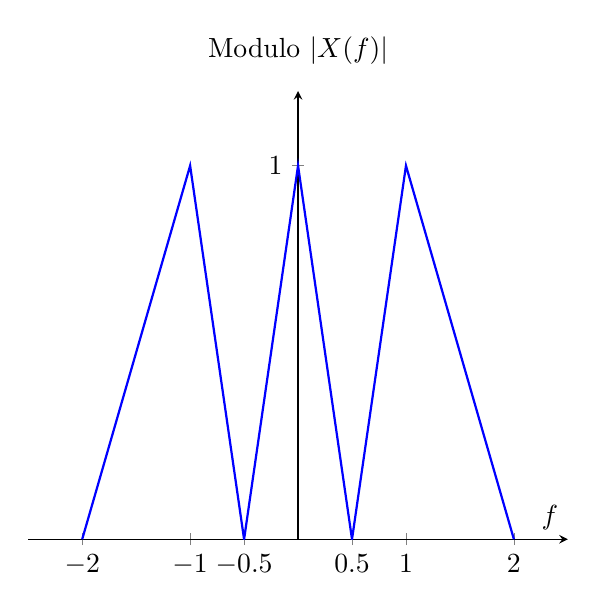
\begin{tikzpicture}
            \begin{axis}[
                title={Modulo $|X(f)|$},
                axis lines=middle, xlabel=$f$,
                xmin=-2.5, xmax=2.5, ymin=0, ymax=1.2,
                xtick={-2, -1, -0.5, 0, 0.5, 1, 2}, ytick={1}
            ]
            \addplot[blue, thick] coordinates {(-2,0) (-1,1) (-0.5,0) (0,1) (0.5,0) (1,1) (2,0)};
            \end{axis}
        \end{tikzpicture}
        \begin{tikzpicture}
            \begin{axis}[
                title={Fase $\angle X(f)$},
                axis lines=middle, xlabel=$f$,
                xmin=-2.5, xmax=2.5, ymin=-4, ymax=4,
                xtick={-2, -0.5, 0, 0.5, 2}, ytick={0, 3.14},
                yticklabels={0, $\pi$}
            ]
            \addplot[red, thick] coordinates {(-2.5, 0) (-2, 0)};
            \addplot[red, thick] coordinates {(-2, 3.14) (-0.5, 3.14)};
            \addplot[red, thick] coordinates {(-0.5, 0) (0.5, 0)};
            \addplot[red, thick] coordinates {(0.5, 3.14) (2, 3.14)};
            \addplot[red, thick] coordinates {(2, 0) (2.5, 0)};
            \end{axis}
        \end{tikzpicture}
        \end{center}
        
        \item \textbf{Spettro del Segnale Ricostruito $X_R(f)$}
        
        La banda del segnale è $B=2$ Hz. La frequenza di campionamento è $f_s=3$ Hz. La condizione di Nyquist ($3 \ge 2 \cdot 2$) è violata, quindi c'è aliasing. La banda base di ricostruzione è $[-f_s/2, f_s/2] = [-1.5, 1.5]$ Hz.
        
        Lo spettro campionato nella banda base è $\tilde{X}_{aliased}(f) = \sum_k X(f-k f_s)$. Dobbiamo considerare la replica centrale ($k=0$) e le code delle repliche adiacenti ($k=\pm 1$) che si sovrappongono.
        \begin{itemize}
            \item Per $|f|<1$: non c'è sovrapposizione. $\tilde{X}_{aliased}(f) = X(f) = 1-2|f|$.
            \item Per $1 \le f \le 1.5$: si somma il contributo di $X(f)$ e di $X(f-3)$.
            \begin{itemize}
                \item $X(f) = f-2$.
                \item Per l'argomento $f-3 \in [-2, -1.5]$, $X(f-3) = |f-3|-2 = (3-f)-2 = 1-f$.
            \end{itemize}
            Sommando i contributi: $\tilde{X}_{aliased}(f) = (f-2) + (1-f) = -1$.
            \item Per simmetria, per $-1.5 \le f \le -1$, si ha $\tilde{X}_{aliased}(f) = -1$.
        \end{itemize}
        Il filtro di ricostruzione $H_R(f)$ ha guadagno $T=1/f_s=1/3$ e taglia a $\pm 1.5$ Hz. Lo spettro ricostruito è $X_R(f) = \tilde{X}_{aliased}(f) \cdot (1/f_s)$.
        
        \[
            \mathbf{X_R(f) = \frac{1}{3} \begin{cases} -1 & \text{per } 1 \le |f| \le 1.5 \\ 1-2|f| & \text{per } |f|<1 \\ 0 & \text{altrimenti} \end{cases}}
        \]
    \end{enumerate}
\end{soluzione}